\documentclass[parskip]{cs4rep}

\usepackage{graphicx}

\usepackage{url}

\usepackage{float}

\begin{document}

\title{An LLVM based compiler from Objective-C to Dalvik Virtual Machine}

\author{Stanislav Manilov}

% to choose your degree
\degree{Computer Science and Mathematics}

% to choose your report type
\project{4th Year Project Report}

\date{\today}

\abstract{
TODO
}

\maketitle

\tableofcontents

%\pagenumbering{arabic}

\chapter{Introduction}

\section{Motivation}

Today we observe a rapidly growing mobile applications market \cite{P1}
that induces equally fast growing demand for high-quality and reliable development
tools. In 2011 the market generated a revenue of \$5.5 bn \cite{P1},
which is estimated to be 6.5 \% of the value of the desktop software market
(please, see Figure ~\ref{fig:softwareMarket2011}). This illustrates the significance of the mobile applications market.

\begin{figure}[h!]
    \centering
        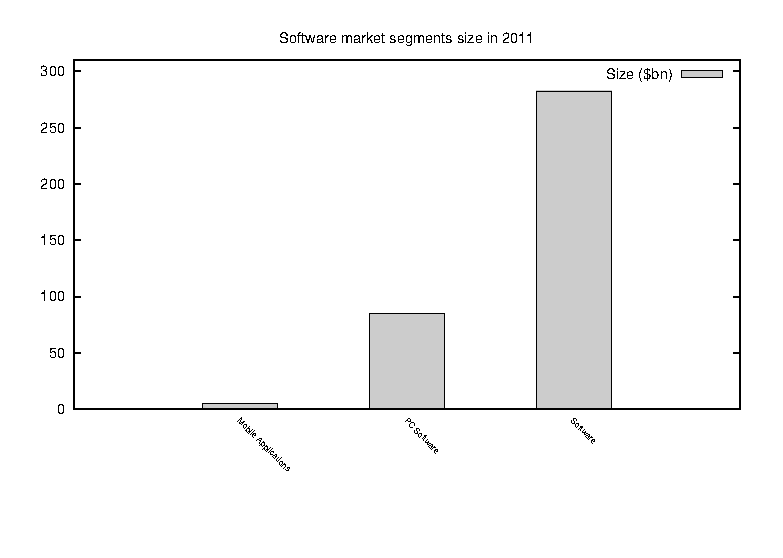
\includegraphics[width=1.0\textwidth]{markets}
    \caption{Software market size in 2011 \cite{P1} \cite{P2} \cite{P3}.}
    \label{fig:softwareMarket2011}
\end{figure}

A main challenge for mobile app developers is producing and maintaining cross-platform applications. Although there are already plenty of tools that address writing such applications (please, see Table ~\ref{tab:crossPlatformTools}), there are three main problems with them:

\begin{itemize}
\item
all of them require learning additional languages (e.g. HTML, JavaScript, or
Lua),
\item
most of them violate the Apple SDK Agreement \cite{P5} \cite{P6} by
producing apps originating from disallowed languages, and
\item
none of them can deal with automatic porting of already existing code that was
originally written for a specific platform.
\end{itemize}

\begin{table}
    \centering
    \begin{tabular}{ | l | p{4.4cm} | p{2.6cm} | p{3cm} |}
    \hline
    Name & Required Knowledge & Cost & Since \\ \hline
    Sencha Touch & HTML, CSS, JavaScript & Free & November 2010 \\ \hline
    jQuery Mobile & HTML, CSS, jQuery & Free & October 2010 \\ \hline
    Tiggzi & HTML, CSS, JavaScript & \$0 - \$180 pm & Unknown \\ \hline
    AppMakr & HTML, CSS & \$79 pm & January 2010 \\ \hline
    iBuildApp & HTML, CSS & \$10 pm & 2010 \\ \hline
    Widgetbox & HTML, CSS & \$25 - \$100 pm & October 2010 \\ \hline
    foneFrame & HTML, CSS, JavaScript & \$0 - \$59 & Unknown \\ \hline
    phoneGap & HTML, CSS, JavaScript & Free & August 2008 \\ \hline
    Corona & Lua & \$200 - \$350 py & December 2009 \\ \hline
    \end{tabular}
    \caption{Comparison of popular cross-platform mobile tools \cite{P4}}
    \label{tab:crossPlatformTools}
\end{table}

These points justify the creation of a compiler that can take the source code of
an iPhone application written in Objective-C and produce an equivalent Android
application. However, there are a couple of major issues with this idea:
firstly, the libraries used for iPhone development - Cocoa API - are proprietary
and thus can not be compiled for Android, and secondly, interface guidelines for
the two platforms differ and thus interfaces can not be literally translated.
Fortunately, there is a community effort to solve the first problem - the
GNUStep project. And while the interface guidelines differ, they are
specific enough to make the detection and translation of idioms possible.

This discussion outlines two of the three major components that a system of the required type must have: a version of the Cocoa API, compiled for the Android platform, and an interface translation module. The third necessary component is, of course, a compiler core that can translate the actual program logic. As building the whole system is an ambitious task for an honours project, it was decided that the effort would be concentrated on research on the program logic component.

\section{Goals}

As outlined in the background section, the goal of this project is to investigate the possibility of building a system, using which, an Objective-C code can be compiled to a Dalvik executable and can be ran on an Android emulator or an actual Android based smart phone. Essential properties of the system are:
\begin{itemize}
\item
correctness: the produced program should be working as described by the source code. More formally, for a given input the program should produce the same output as native programs compiled by the Gnu Compiler Collection (gcc) and Clang+LLVM, where the two agree;
\item
speed: the time to build a typical program should be acceptable (in the order of minutes at worst).
\end{itemize}

In addition to these, it is desirable that the resulting system has the following properties:

\begin{itemize}
\item
performance of produced code: the produced program should be reasonably fast (same order of magnitude), when compared to an identical program, written in Java and built using the standard tool chain (Android Development Kit);
\item
size of produced code: the size of the produced program should be reasonably small, when compared to an identical program, written in Java and built using the standard tool chain.
\end{itemize}

TODO: finish and link with conclusion

\section{Overview}

a few words on the scope of the implementation: only ints, single modules, assumes int main function, no input, simple output

\chapter{Background}

\section{Objective-C}

Objective-C was originally developped between 1981 and 1983 by Brad Cox and Tom Love as a superset of the C programming language that was strongly inspired by Smalltalk and incorporates its object oriented model\cite{Biancuzzi2009}. The creators of the language concentrated on building an extension that relies on run-time libraries and dynamic binding to improve the ease of integration of different components, rather than inventing a complex powerful software manufacturing system from scratch, which is the approach taken with C++.

The Objective-C language implements the object-oriented paradigm in a different way than the more widely used and successful C++ language. The former's object oriented model is based on Smalltalk, as previously mentioned, while that part of the latter is modelled after the aproach taken in the Simula language. As a result of this, even though the two languages are good at tackling similar domains of problems, their core principles are different. Objective-C was designed with simplicity in mind - the language architects aimed at adding the absolute minimum of additional features that would enable the programmers to write object-oriented programs. Backward compatibility with C and understandability were also main objectives of the project. In contrast, Bjarne Stroutstrup (the creator of C++) wanted to create a language for maximum efficiency that allowed him and fellow collegues to "express program organisation as could be done in Simula"\cite{Biancuzzi2009}. The focus was on power and speed, and as a result C++ turned out to be more complex and harder to understand than Objective-C. However, in the long run it also turned out to be more popular, the reason for which the Objective-C creators find in the fact that C++ was given away for free by AT\&T, rather than in actual benefits of the language. The compiler and support libraries of Objective-C were the only revenue sources of Stepstone (the company of Love and Cox), so they couldn't afford to open source the project, and thus it remained mostly unpopular.

The first notable recognition of the language was when it was chosen as the native language for the NeXTStep 1.0 operating system in 1989 - the first mature operating system of NeXT Computer. It is hard to find the reasons for choosing Objective-C over C++ in that setting. A propaganda NeXTStep manual from 1992\cite{NeXTCorporation1991} claims that NeXT chose Objective-C for its ease of learning and because of its support for dynamic binding, arguing that the latter allows for more seemless updates of the system, but this can be achieved equally easy by using shared/dynamically linked libraries. The author speculates that a major part of the decision was the need to differentiate from other OS vendors of the time and create a NeXT specific developer community and user base. Whatever the reason, the result remains and it is a popularisation of the Objective-C language.

NeXT later acquired the rights over Objective-C in 1995 and became the main advocator of the language. The company itself was acquired by Apple Inc. in 1997 and the NeXTStep operating system eventually evolved into what became known as Mac OS X over the period of four years. This way Objective-C propagated its way into the Mac computers of today. Native Mac apps are developed using the proprietary Cocoa API, which is written in Objective-C. A mobile version of this API - Cocoa Touch - is what is used for developing applications for the iPhone, iPod, and iPad.

Since programming in the past couple of decades has not been restricted to a selected few, but rather an essential skill sometimes compared to literacy in its importance, NeXT/Apple have recognised that they need to provide the general public (rather than only Mac users) with tools that allow creation of Objective-C programs if they want to make Objective-C a competative and popular language.

The first such initiative was OpenStep which was an object-oriented API for non-NeXTStep operating systems. The GNUStep project is an open source implementation of Cocoa that is based on OpenStep. Later, a team of NeXT/Apple engineers, lead by Steve Naroff developed the GCC Objective-C frontend. However, it relied on run-time libraries, which were not open sourced, so this effort remained useless to the general public. Finally, Apple invested in building the Objective-C frontend to Clang in 2007, which enabled the author to undertake this project.

Thanks to the existence of Clang, the reader need not understand the minute details of the Objective-C language as it is translated by this LLVM frontend to LLVM bytecode.

\section{LLVM and Clang}

\subsection{History}

LLVM was initially concieved as "a compilation strategy" that was designed to provide "effective multi-stage optimisation and more effective profile-driven optimisation, and to do so without changes to the traditional build process or programmer intervention"\cite{Lattner2002}. It was started as the Masters Thesis project of Chris Lattner under the supervision of Professor Vikram Adve in the year of 2000 at the University of Illinois at Urbana-Champaign. The main goals were to lay the foundation of a modern modular compiler, that has similar interface to its contemporaries and predecessors. The paper was published in 2003, and the LLVM infrastructure was open sourced, subsequently being widely adopted by the community and researchers\cite{Lattner}. In 2005, Apple hired Lattner to work at their compilation team and during the following seven years he advanced in positions to reach that of "Director and Architect, Developer Tools Department" in January 2013. Now he is responsible for the management of the entire Developer Tools department at Apple[cite http://www.nondot.org/sabre/Resume.html]. Apart from an example of impressive personal development, this is important for the evolution of LLVM, as during his career at Apple Lattner has mainly been working on LLVM and related tools, including Clang.

\subsection{Structure}

There are four stages of compilation included in LLVM: pre-linking compilation, link-time optimisations, run-time optimisations, and offline optimisations\cite{Lattner2002}. The first two stages are common in traditional compilers and include static analysis and classical optimisations. After stage two, the program is compiled to machine code, but high-level type information is also included in the output. This is one of the key novelties in LLVM, as this information is later used to perform the run-time optimisations and offline optimisations.

During execution of an LLVM compiled program, profile information is gathered from the usage statistics. This is different to the usual approach of profiling, as the usage information is actual, user specific data, rather than synthetic data that is fabricated by the developer. This way, the pitfall of profiling for the wrong data is avoided and the increase of performance is higher. In addition to this, the whole profiling process is automated and the overhead of effort is removed. 

Other activities that take place during execution of the program are run-time optimisations. These are optimisations that can be found in standard Just-In-Time (JIT) compilers, but also optimisations that use the profiling data to make common cases in the code faster, for the price of slowing down less common control flow paths. If there are profile driven optimisations that are too expensive to perform, they are sheduled for the offline optimiser.

The offline optimisations in LLVM are more aggressive dynamic optimisations that are too expensive to run alongisde the program, so they are performed when the system is idle. They are particularly useful for programs in which the majority of time of the execution is spent over a large part of the code, rather than having a particular 'hot' spot. In such cases the profiler would detect optimisation opportunities, but it would not be beneficial to actually perform them in run-time, so they are delayed to when the offline optimiser can step in.

\subsection{Language} \label{sec:LLVMLanguage}

The instruction set that LLVM uses provides an infinite amount of typed virtual registers in Static Single Assignment (SSA) form, which hold values of primitive types. The primitive types include integers, floating point numbers, and pointers. The types relevant to this project are:
\begin{itemize}
\item iN - an integer of N bits;
\item half, float, double - different formats for floating point numbers, the first three being 16 bit, 32-bit, and 64-bit floating point representations.
\end{itemize}

Memory is accessed via the store and load operations and is partitioned in global area, stack, and heap. Stack variables are allocated using the alloca instruction and are freed automatically when the function returns. Heap variables are allocated using malloc and need to be freed explicitly using the free instruction. In this way, the memory management in the LLVM language is similar to that in the C programming language.

The arithmetic and logical operations are in three-address form. The available arithmetic operations are: add, sub, mul, div, and rem. The names are self explanatory and correspond to the usual operations in arithmetic. Div and rem are whole number division and remainder functions. The available logical operations are: not, and, or, xor, shl, and shr.

Additionally, there is the comparison instruction 'icmp' that produces a boolean result and takes as first argument the type of the comparison: eq, ne, lt, gt, le, and ge. Respectively, they stand for 'set-on-': equal, not equal, less than, greater than, less than or equal, and greater than or equal. Other instructions can take 0, 3, or a variable number of arguments, examples for which are the call instructions and the SSA phi instruction.

All instructions in the LLVM instruction set are polymorphic. This means that they can operate on different types and do not need to have special versions for each of the possible types. The types of the operands also define the semantics of the instruction.

\subsection{Modifying LLVM}

In order for one to be able to modify and add features to LLVM, they must understand a few basic concepts of the code and its structure.

The Value class is fundamental in LLVM. In most basic terms everything is a Value within the world of LLVM. This includes obvious things, like the classes Constant, GlobalValue, and Instruction, but also includes BasicBlock, ConstExpr, and even Function \cite{P9}. It is the base class of all values that need to be computed or passed as arguments to other values. It also provides basic methods for identifying and differentiating between values, e.g. hasName, getValueName, and getValueID. All Values have a Type, which is one of the few classes which are not subclasses of Value. Changing the name of a Value updates the symbol table of the Module that owns it. Finally, each Value has a list of User objects (User inherits Value), which tracks the other Values that use it, e.g. Functions or ConstExpr's.

The Type class is in the base of another hierearchy - the type hierarchy in LLVM \cite{P10}. The header file that defines the hierarchy is not too straightforward to find, so the author feels obliged to point to it: llvm/DerivedTypes.h. There is a single instance of each Type, and thus comparison of types is straightforward. Uniqueness of instances is maintained by creating these instances in static factory methods and never freeing them, once they are created. Examples of members of the Type class hierarchy are llvm::IntegerType, llvm::PointerType, and llvm::FunctionType.

Other important concepts are that of Contexts and Modules. Quite self explanatory, a Context describes the execution state of LLVM. Different Contexts can exist at the same time and can run in parallel on multiple threads, however single Contexts are not guaranteed to be thread safe. They are created via the LLVMContextCreate method and freed via the LLVMContextDispose method. If the second is omitted a memory leak would occur, so the programmer needs to make sure that every LLVMContextCreate method is paired with a LLVMContextDispose method. The topic of Modules is touched upon in the next subsection.

\subsection{Building a new backend} \label{sec:buildingANewBackend}

Because of the high modularity of the architecture of LLVM it is possible to build new backends and plug them in relatively easily. A backend is basically a module that takes the LLVM internal representation and translates the program to a specific target native code. Since Clang includes an Objective-C frontend for LLVM, the author concentrated on developing only a backend that produces Dalvik bytecode from LLVM internal representation. Once the backend was working, it was possible to produce Dalvik programs from Objective-C code, by passing the code to Clang, and setting it so it emits LLVM bytecode to a file. This file is then given to the backend, which produces Dalvik assembly code (smali), which is assembled using the apktool utility provided by Google, and installed on a testing device.

There are different ways to create the backend depending on the amount of the recommended structure that the developer wants to incorporate in it. Ideally, it should extend a large number of LLVM classes and provide target specific details\cite{P8}. This way more of the previously discussed LLVM features can be enabled. However, if the aim is to simply get a working prototype, it is sufficient to extend only a few classes and then to register the backend within LLVM.

Also, work in LLVM is done in passes of different modularity (block, function, or module), and the developer that is extending the functionality can decide which one (or more) of those they want to implement. However, when writing a backend it is obvoius that the whole program needs to be processed, so writing a module (the largest granularity) pass is sufficient.

For example, if one wishes to create a new target called 'Blank', they must create a new subdirectory in llvm/lib/Target with the name of the target. This folder will contain the new backend implementation which typically includes classes for different modules of the backend, e.g. a module for parsing assembly, one for JIT compilation, one for printing instructions, etc. However, a minimum working implementation can be achieved by only extending the TargetMachine class of LLVM. Continuing with the example, one would create a file BlankTargetMachine.h in the folder and create a skeleton extension of the TargetMachine class (the CppBackend target is a good example of how to do this.) The key method is addPassesToEmitFile, which would be used to create a simple static compiler. We will return to this later.

As mentioned previously the work in LLVM is done in passes, the most general one being the module pass. It is represented by the ModulePass class of LLVM. In order to continue with the creation of the new target one needs to create a file Blank.cpp in the Blank folder, containing a class extending the ModulePass class.

There is a single most important method of the class ModulePass that needs to be implemented and this is the runOnModule method. It takes a reference to an LLVM Module object as an argument and returns whether the there were any problems during the run ('true' if so, and 'false' on success). The LLVM Module object represents all the information that is contained in a single file of LLVM bytecode. The data is split to functions, which are further split to basic blocks of control flow, and the basic blocks are comprised of sequences of instructions. Thus a simple static compiler for a target architecture  can be implemented by traversing the Module object and outputting assembly code for this architecture. Depending on how similar this code is to LLVM's internal representation the difficulty of this step can range from moderate to impossible, but for most standard architectures (including Dalvik VM) it is a good starting step. Thus, after implementing the runOnModule method (and quite probably a set of helping methods to maintain high modularity and readability of the code) the person writing the backend should have a solid foundation for testing.

Once the extension of the ModulePass class is implemented, it is plugged in the system by adding it to the PassManagerBase of the newly created target. This is done in the addPassesToEmitFile method mentioned earlier. This method can be implemented in the Blank.cpp file and can also include conditionals to add different passes, depending on the arguments of the function, but this is optional.

Now the implementation of the example backend is complete, it needs to be registered with LLVM in order for it to be included in llc - the executable that compiles LLVM bytecodes for a specified architecture. This is usually also done in the Blank.cpp file, writing an external C function that simply instantiates the LLVM RegisterTargetMachine template with the type argument being BlankTargetMachine. The instantiation seemlessly triggers the registration mechanism and nothing else needs to be explicitly done.

Other formalities that need to be carried out before the Blank backend can be successfully built are:
\begin{itemize}
\item
creating a TargetInfo subfolder containing a single file BlankTargetInfo.cpp. This file has to declare and register the llvm::TheBlankTarget object of type Target in a similar fashion to the registration of the BlankTargetMachine class;
\item
creating CMakeLists.txt, Makefile, and LLVMBuild.txt files that will instruct the build system how to handle the new target. Also adding Blank in subdirectories in llvm/lib/Target/LLVMBuild.txt;
\item
adding 'Blank' to \verb|TARGETS_TO_BUILD| and \verb|a_target| switch in llvm/configure; note that in order for this to work, this token should be the same as the one in LLVMInitializeBlankTarget.
\end{itemize}

Once these final steps are done, the Blank backend should be working. To test that this is the case, one should rebuild the llc project and run llc with option march as 'blank'.

\section{Android and Dalvik}

\subsection{History}

Android was revealed on the 5th November 2007 by Google, when they introduced the Open Handset Alliance (OHA)\cite{DeLacey2007}. The alliance comprises of several dozens of telecommunication companies and their aim is to produce more open and customisable mobile phones. The major product to achieve this is Android - an open source mobile operating system based on Linux.

Historically, the development of the Android operating system starts around 2003 at a company called Android Inc\cite{BloombergBusinessweek2005}. The project is developed under high secrecy and little is known about its existence before it was introduced in 2007, apart from the fact that the company engaged with it was acquired by Google in 2005.

Android entered a market that was dominated by conservative vendors: Apple, Microsoft, and RIM. Their philosophies don't reserve a place for the idea of open-source software and this is what was different about the new operating system. During the following five years the community of programmers developing Android apps grew rapidly, producing around 700 000 apps for the platform\cite{Islam2012}. Today Android is the most popular mobile operating system, owning three quarters of the market share\cite{IDC2012}.

In addition to advocating open-source, Android has the advantage that it allows hardware manufactures to concentrate on improving the devices and not worry about the software that runs on them. This way it is very useful for new companies that don't have the financial or technical resource to develop their own operating system. As a result, Android is even employed in devices it was not originally intended for, like TV sets and game consoles\cite{Telecompaper2012}\cite{Etherington2013}.

\subsection{A 'Hello World' Android app} \label{sec:AndroidHelloWorld}

The simplest Android app has an extension of the Android Activity class as its entry point. It also contains a lot of configuration and resource files, but only the Activity class is relevant to this project. There is a main such class for the app, specified in the AndroidManifest.xml file in the root of the source tree. When the app is started on a device, the onCreate method of this class is invoked, and it usually configures the app and displays the initial screen of the app. This is used as an entry point for programs compiled with Objective-Droid (see section \ref{sec:Implementation}).

\subsection{Dalvik}

Dalvik is the virtual machine (VM) that runs on Android devices. Since Android applications are written in Java, Dalvik is similar to a Java Virtual Machine (JVM), but has several key differences.

First of all, Dalvik is register based, compared to the stack based JVM. This means that arguments for the instructions reside in virtual registers (a total of 65K of them) and not on a stack. Thus, the push and pop instructions that are used to manipulate the stack in order to execute stack based operations can be removed, resulting in less instructions, and thus smaller programs - important improvement for mobile applications.

Secondly, Dalvik does not use the defaut Java GUI frameworks (i.e. AWT or Swing) but rather relies on a dedicated one. However, open source frameworks have been successfully ported to run on Android, notably the popular Qt framework, so it is still possible to write applications which are independent of the VM  used.

Most importantly though, due to the subtle differences between the Dalvik bytecode and the Java bytecode, Dalvik has its own file format - .dex. The .dex files are usually compiled from Java .class files using the dx tool from the Android SDK. However, the different file format further distantiates the two virtual machines and makes them incompatible in the strict sense.

\subsection{Instruction Set} \label{sec:DalvikInstructionSet}

The instruction set of Dalvik (Dalvik bytecode) is surprisingly different than Java bytecode. This is mainly due to the fact that the Dalvik virutal machine is register based, rather than stack based like the Java virtual machine. Thus, for example, there are no load/store or push/pop instructions in Dalvik to manage a stack. There are about 65 thousand 32-bit virtual registers at the programmer's disposal. Double precision floating point numbers and 'long' integers are stored in a pair of neighbouring registers. They do not need to be aligned, e.g. can be the pair {v2, v3} or the pair {v17, v18}.

The types in Dalvik are:
\begin{itemize}
\item int - a 32 bit integer;
\item long - a 64 bit integer;
\item byte - an 8 bit integer;
\item char - a character;
\item float - a 32 bit floating point number;
\item double - a 64 bit (double precision) floating point number;
\item and boolean - a boolean value (true or false).
\end{itemize}
Internally, all the values are represented by numbers: integer constants are trivial, characters are represented using the UTF-16 encoding, and booleans are either 0 for false, or 1 for true. It gets more complicated when floating point numbers are involved. Reverse-engineering has shown that 'float' and 'double' values are in 32 bit and 64 bit IEEE-754 format respectively.

Arithmetic and logical operations are in three-address mode\cite{TheAndroidOpenSourceProject2007} (the general form of a binary operation is 'binop vAA, vBB, vCC') which is the same as in LLVM's internal representation. However, arithmetic and logical operations in Dalvik's instruction set are not polymorphic, e.g. there are four versions of add: add-int, add-long, add-float, and add-double. There are also versions for when one of the operands is a literal, and versions taking only two registers. This flexibility allows for selecting the minimum amount of instructions in each context and thus achieving the desired reduction of program size, but leads to complications when translating the polymorphic LLVM instructions.

Another important difference between Dalvik bytecode and LLVM IR to note is that there are no boolean comparison operators in Dalvik. There are two alternative ways to compare numbers. One option is to use the comparison operators in Dalvik, which return -1, 0, or 1, for 'less than', 'equal', or 'greater than' results respectively. This option is further complicated by the fact that the arguments to these instructions can only be of type long, float, or double - in other words anything but an integer - so if integers have to be compared, they have to be cast to longs before that can be done. The other option is to use the family of conditional branching instructions: if-eq, if-ne, if-lt, if-gt, if-le, and if-ge. However, using this approach two labels need to be added to the code, complicating the control flow. The difference of the two approaches is examined in the implementation section.

Finally, there are two other classes of operations relevant to this project: move and const. The two have generally the same purpose - copying a literal or the contents of another register to a register. There are 13 variants of move, each specific for a different situation and there are 11 variants of const.

TODO: Bjoern: In section 2.3.3 you could include a table with Dalvik instructions and a short (one-line) description.

\chapter{Design and Implementation}

\section{Design}

\subsection{Overview}

Before the commencing of the work on the project, it was agreed that the best approach is to base the system on the LLVM compiler infrastructure. There are multiple advantages that come with building upon LLVM:
\begin{itemize}
\item
Firstly, LLVM comes with Clang - a complete frontend for languages based on the C programming language. These include Objective-C, so basing Objective-Droid on LLVM removed the need of producing front-end components like a parser or a lexer.
\item
Secondly, LLVM comes with a powerful middle end that contains a wide range of optimisations\cite{P7}. Including these optimisations in Objective-Droid proved to be highly beneficial for the quality of the output. 
\item
Thirdly, using an established compiler infrastructure as a foundation provided an interface that developers are already used to, at no additional effort cost. This would reduce the learning curve for users of Objective-Droid and let them feel more confident about using the tool.
\item
Fourthly, building a backend for LLVM by the guidelines allows it to be contributed back to the project. This allows all (or parts) of Objective-Droid to be given back to the compiler developing community easier than if it was being developed from scratch.
\end{itemize}

The first essential component of the Objective-Droid system is the LLVM backend. The target code is Dalvik bytecode (sometimes called smali code), as there are already assembling tools for it that produce Dalvik binaries.

The second essential component is a packager that given the smali code assembles it, packages it, and signs the package. This would allow the package to be installed and tested on an emulator or a phone.

The final component of the Objective-Droid system is a wrapper program or a script that automates the whole process of compiling, packaging, and possibly installing the program on a phone. This script would be useful for testing, but is not mandatory.

For a summary of the design, please see Figure ~\ref{fig:design}.

\begin{figure}[htp]
    \centering
        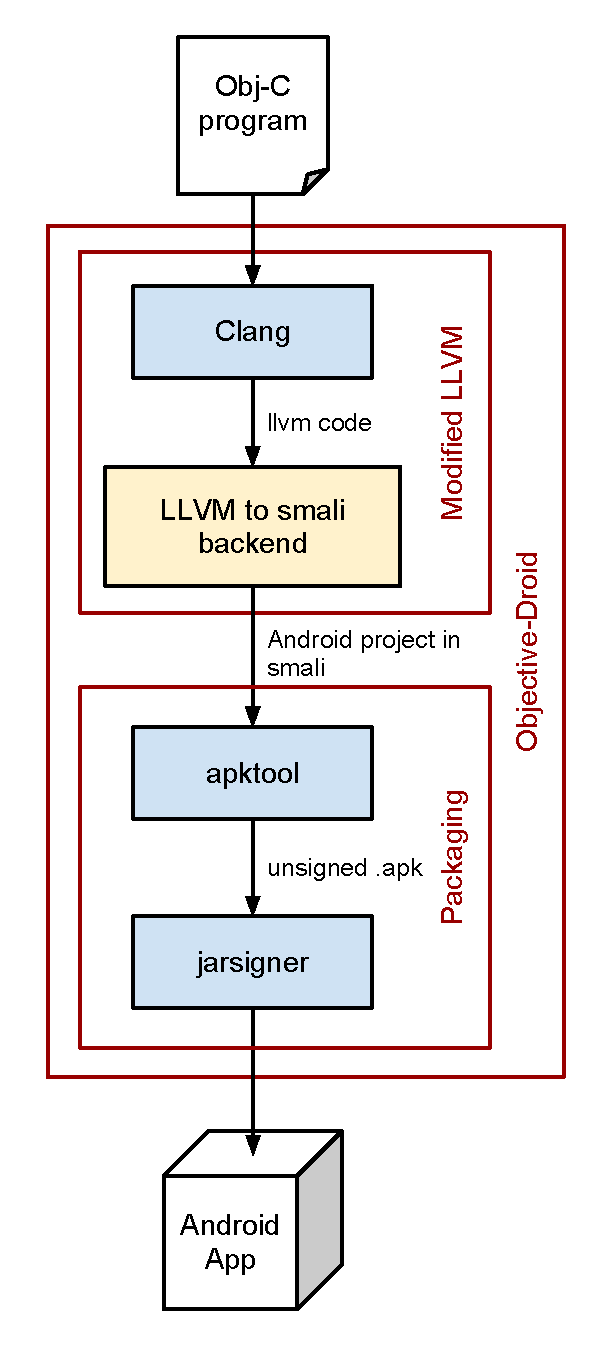
\includegraphics[width=0.6\textwidth]{design}
    \caption{Overall design of the Objective-Droid system.}
    \label{fig:design}    
\end{figure}

\subsection{Design of the backend} \label{sec:designOfTheBackend}

Initially, an attempt to design the backend by the formal guidelines\cite{P8} was made, but this proved overly complicated and at the end - unnecessary for this particular project. The reason for this is the fact that Dalvik VM is a virtual machine, and not an actual physical architecture. It has its own runtime optimisations (e.g. JIT compilation) so leveraging LLVM's optimisation power is not a necessity and thus a prototype implementation can go by without many of the recommended classes, for example AsmParser, Dissasembler, JIT, or Scheduler. Furthermore, as the architecture is relatively young - less than ten years have passed since its inception - there is only one variant of it, so there is neither need to build the backend in a way that supports different subtargets (no need to implement the Subtarget class).

This reduction in boilerplate code allowed for rethinking of whether the guidelines should be followed. An alternative approach was adopted and the backend was designed to include only the most important basic functionality. To favour simplicity it was implemented in a single main class and a few supporting files, as discussed in subsection \ref{sec:buildingANewBackend}. This simplicity gave the advantage of easier configuration and acquiring a working prototype faster. This design proved sufficient for implementing a static single-pass backend that mainly relies on a lookup table for substituting LLVM instructions with single Dalvik instructions or a sequence of them.

\section{Implementation} \label{sec:Implementation}

\subsection{File structure}

As apparent from the design outline, the most integral part of the project is building the LLVM backend.

An LLVM backend needs to be implemented as a subclass of the LLVM TargetMachine class \cite{P8}. Depending on the features of the target architecture, the implementation needs to provide a suite of files. E.g. if MIPS is the target architecture, the implementation needs to provide files that describe: the instructions, the registers, the interface for JIT compilation, etc. On the other hand, if the target is not a real architecture, but rather a high-level language (which is the case of the backend that produces C++ code) the implementation can be as simple as a single class.

As argued in section \ref{sec:designOfTheBackend}, a simple implementation is sufficient when targeting Dalvik bytecode, thus the second approach examined in section \ref{sec:buildingANewBackend} was taken. The implementation of the backend for Objective-Droid resides in a subfolder of llvm/lib/Target called Dalvik. The Dalvik folder (Figure ~\ref{fig:dalvikFolder}) contains: 
\begin{itemize}
\item Dalvik.cpp - the main file which contains the implementation of the ModulePass class (called DalvikWriter), the implementation of the addPassesToEmitFile method of the Target class (called DalvikTargetMachine), and the static LLVMInitializeDalvikTarget method that registers the TheDalvikTarget object (instance of Target) with LLVM;
\item DalvikTargetMachine.h - definition of the DalvikTargetMachine class, and declaration of TheDalvikTarget object;
\item configuration files - CMakeLists.txt, LLVMBuild.txt, and Makefile;
\item the TargetInfo subfolder - contains a file describing the Target for documentation purposes and configuration files for the build system.
\end{itemize}

\begin{figure}[htb]
    \centering
        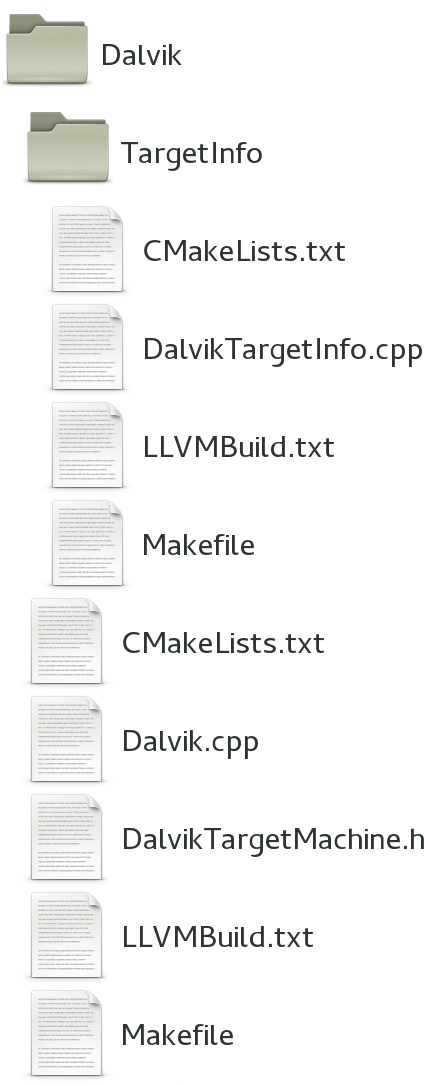
\includegraphics[width=0.24\textwidth]{dalvik-folder}
    \caption{Dalvik folder structure.}
    \label{fig:dalvikFolder}    
\end{figure}

\subsection{Target class}

The Target class is the entry point of the Objective-Droid backend. As described earlier, it is the standard mechanism of adding a backend to the LLVM infrastructure. When LLVM performs the static part of the compilation, it first translates the source to LLVM bytecode (using Clang), optimises the program, and then the target chosen by the command line option 'march' is invoked. This invokation is done by calling the passes that were registered by one of the 'addPassesToEmit...' functions. In the case of this project, this is the addPassesToEmitFile function.

The role of this class in Objective-Droid is simply to act as the link between the LLVM infrastructure and the ModulePass class, which is used to implement the bulk of the backend. In general, the Target class can be used to do more, but this is enough for the purposes of the project.

\subsection{ModulePass class} \label{sec:ModulePassClass}

The main class of the implementation inherits the ModulePass class of LLVM. The ModulePass is typically used for passes that manipulate the whole program, thus it serves the needs of the Objective-Droid backend. The runOnModule method is the entry point of the class. This method is given a description of the program in a Module object as an argument and returns 'false' on success.

The implementation of the runOnModule method simply builds an Android Activity class corresponding to the module passed to the compier. Multiple modules are not yet supported. The Activity class is built by first printing out prelude boilerplate code that includes a package declaration, specifies the parent class (android.app.Activity), and adds a declaration of the source file. Next, the list of global variables is iterated over and a static field with the corresponding type is created for each of them. 

This is where the first difficulty arises: the types supported by the LLVM bytecode and the Dalvik bytecode are different. As mentioned in section \ref{sec:LLVMLanguage} LLVM can specify integers of any size, unlike Dalvik, where integers can only be 8, 16, 32, or 64 bit wide. Characters in the two representations are not compatible as Clang compiles char values to 8 bit integers (as per C standard), and Dalvik uses 16 bit integers (as per Java standard). Finally, Dalvik has no notion of 16 bit floating point numbers, so the variables declared as such in the LLVM bytecode have to be implemented as 32 bit floating point numbers.

Table \ref{tab:typeConvertion} summarises how LLVM types are converted to Dalvik types. This convertion tries to maximise the utilisation of different Dalvik types while maintaining correctness. Only the integer part of the convertion was implemented, however. Implementing the floating point part would be pointless without an emulation of the IEEE-754 standard, as floating point constants need to be represented in it. The author decided to focus on making a prototype working with integers and thus spared himself the effort of implementing the standard and thus floating point numbers. For a complete implementation of the LLVM language the other types need to be emulated in dedicated classes.

\begin{table}[htb]
    \centering
    \begin{tabular}{ | l | l |}
    \hline
    LLVM type & Dalvik type \\ \hline \hline
    i1 & boolean \\ \hline
    i8 & byte \\ \hline
    i16 & char \\ \hline
    i32 & int \\ \hline
    i64 & long \\ \hline
    other iN & error \\ \hline
    half & float \\ \hline
    float & float \\ \hline
    double & double \\ \hline
    other type & error \\ \hline
    \end{tabular}
    \caption{Dalvik types corresponding to LLVM types}
    \label{tab:typeConvertion}
\end{table}

In addition to creating a static field with the corresponding type for each of the global variables, information about the variable (name, type, and initial value, if any) stored in a table of fields during compilation. Despite arrays being generally unsupported, the special case of a string (an array of characters) is. Strings are treated specially because they are a requirement for output operations in Objective-C - the first argument of the printf function needs to be a string literal.

After the global variables have been translated to fields, the ones that are statically initalised in the Objective-C code need to be initialised in a "static constructor" of the Activity class. The static constructor is the compiled version of a Java static initialisation block. Thus, the next step of the compilation the creation of this constructor, using pairs of 'const' and 'sput' instructions to implement the initialisation of each of the fields. This is implemented as printing out constant header and footer strings for the constructor, and running a loop in between that prints out the mentioned pairs of instructions. Regarding strings - the fields are declared as being of the type java.lang.String, and constants are loaded by the surprisingly convenient instruction 'const-string'.

Once the global variables have been dealt with, the turn of the functions comes. Objective-C functions are translated to public static methods in Dalvik. Each of the functions is printed similarly to the previously discussed static constructor: there is a header string that contains the name and type of the function, and a footer string that declares the end of the function. In between, the list of instructions are translated and printed, grouped in basic blocks. For details about the translation of instructions, please see section TODO\ref{sec:instructionTranslation}.

Finally, when all the functions are translated, the onCreate method is printed. As explained in \ref{sec:AndroidHelloWorld}, onCreate is the standard way of starting up an Android Activity. The boilerplate code for the onCreate method includes an invokation of the super constructor, a call to the 'finish' method of the Activity class, and a return instruction. The call to the 'finish' method stops the application from displaying a screen to the user, as testing is done via the 'adb' debugger, provided by Google. The prototype implementation assumes that the Objective-C program contains a 'main' function of type 'int', and thus an invokation to the method representing this function is the single instruction output in the body of onCreate.

\subsection{Instruction Translation} \label{sec:instructionTranslation}

The functions are translated by iterating over the instructions in them and translating each instruction separately. Some LLVM instructions have quite close equivalences in Dalvik bytecode, for example the 'ret' instruction. Others, as mentioned previously, need short sequences of Dalvik instructions to emulate them, for example the boolean comparison operators. The symbol table is implemented as a map from variable names to registers called VarsRegsMap. 

A single function is called when an instrution has to be translated. It checks the opcode of the instruction and depending on that calls specific code for each instruction. A subsection describing each instruction translation follows.

\paragraph{The 'ret' instruction} "... is used to return control flow (and optionally a value) from a function back to the caller. There are two forms of the 'ret' instruction: one that returns a value and then causes control flow, and one that just causes control flow to occur."\cite{P11} The version that just causes control flow to occur is 'ret void' and has an exact equivalent in Dalvik bytecode: return-void. Thus the translation of this version is just outputting this equivalent.

The version that returns a value can either return a constant or a register. In Dalvik, however, there is not a version of 'return' that takes a constant as an argument, so in order to simulate this version the constant has to be loaded in a register using the 'const' instruction, and then returned using the return instruction. Furthermore, if the constant is not of type 'int' (notably, if it is of type representing a floating point number), it might need to be converted to its integer representation by the compiler. As mentioned before, the author has decide to exlude this feature for the benefit of simplyfying the prototype.

Similarly, only registers containing single-word values can be currently returned. The reason for this is that registers containing double-word values need to be returned by the 'return-wide' instruction, and objects need to be returned via the 'return-object' instruction. It was unnecessarry to add this functionality, as the goal was to create a prototype that deals with integers only.

\paragraph{The 'alloca' instruction} "... allocates memory on the stack frame of the currently executing function, to be automatically released when this function returns to its caller. The object is always allocated in the generic address space (address space zero)."\cite{P11} Since there is no explicit stack in Dalvik, this was translated to just reserving a register for later use by adding an entry to the symbol table. The name of the LLVM register that the pointer to the stack memory is assigned to is sanitised and used as key in the new entry in the symbol table. This way, when the name of the LLVM register is later refered to in the LLVM code, the corresponding register will be used, and this would provide the same behaviour as allocating memory on the stack.

An important thing to note is that if the type of the memory to be allocated is different than a 32 bit integer, this translation will yield an incorrect result. Again, as explained earlier, the author was not concerned with this, as the main objective of the prototype is to be compatible with single-word integers. This note is valid for all of the following instructions.

Adding support for more types boils down to allocating a pair of registers for values that need to be represented by 64 bits. In the case of allocating arrays, the 'new-array' instruction has to be used. If irregular types have to be implemented, for example 20 bit integers, the only way to this is to write a class that emulates this behaviour. This is also the case for pointers. Once these type classes are implemented they are allocated with the 'new-instance' instruction.

\paragraph{The 'store' instruction} "... is used to write to memory."\cite{P11} The implementation of this instruction first looks up the name of the Dalvik register that has been reserved for the name of the LLVM register. Then, depending on whether a constant or the contents of another register have to be stored, a 'const' or 'move/16' instruction is printed.

Choosing 'move/16', rather than just 'move' was done in order to support all possible of registers - 'move/16' can have 16 bit arguments, thus can address any of the 64K registers. Unfortunatelly, there is no such variant of 'const', so if this functionality needs to be added the constant can be stored to a pre-reserved low-addressed register - say vFF, and then moved to a high-addressed register via the 'move/16' instruction.

Methods of storing different kinds of values have not been explored as a part of this project.

\paragraph{The 'load' instruction} "... is used to read from memory."\cite{P11} It is implemented in Objective-Droid very similarly to the 'store' instruction. However, it is simpler, as neither of the arguments can be a constant. The name of the source and target LLVM registers are used to look up their respective Dalvik registers and a single 'move/16' instruction is output.

\paragraph{Binary arithmetic operations} There are five binary arithmetic operations that are implemented as a part of this project: 'add', 'sub', 'mul', 'sDiv', and 'sRem'. They stand for sum, difference, product, signed quotient, and signed remainder of division, respectively. The arguments they take need to be of the same type, which can be either an integer or a vector of integers, where only the first one is supported in Objective-Droid.

These instructions are implemented in a common function, which takes the type of the operation as an argument and prints the instruction. The first thing that is done is allocating a new register on the symbol table that would store the result. LLVM creates a new unique register every time it needs to perform a binary operation, so this name can be used to reserve a Dalvik register.Then, the types of the arguments are checked, and three cases are considered: having two constants, having a constant and a variable, and having two variables.

The foremost case is rather unlikely to occur, as the optimisation passes of LLVM are likely to have dealt with it and summed up the constants rather than passing the add instruction on. However, the case was added for symmetry and completeness of binary operations.

In order to add a constant to a variable in Dalvik, the constant needs to be loaded in a temporary register, as there is no add instruction that takes a constant as an argument. Thus, if the second of the three cases occurs, a temporary register is allocated on the symbol table, and a 'const' instruction that stores the constant in this register is printed. It is then used as if it was the second variable supplied.

In the third case (that is - being provided with two variables), the corresponding Dalvik registers are loaded from the symbol table. There is a Dalvik instruction corresponding to each of the mentioned LLVM instructions ('add-int', 'sub-int', 'mul-int', 'div-int', and 'rem-int' respectively). This is printed out, together with the names of the two argument Dalvik registers. Finally, any temporary registers are deallocated, which in practice is removing them from the symbol table, and marking them as available.

Adding support for vector arguments would need to be implemented in a special class. However, adding support for floating point numbers, would be rather straightforward, as this implementation is not integer specific.

\paragraph{The 'icmp' instruction} "... returns a boolean value or a vector of boolean values based on comparison of its two integer, integer vector, pointer, or pointer vector operands."\cite{P11} As explained in \ref{sec:DalvikInstructionSet}, this instruction has no close equivalent in Dalvik. The author has identified two possible approaches of solving this problem: either using the Dalvik comparison operators that return -1, 0, or 1, for 'less than', 'equal', or 'greater than' results respectively, or using the family of conditional branching instructions: if-eq, if-ne, if-lt, if-gt, if-le, and if-ge.

The first approach appears more natural, as it uses the instructions that are designed to be used for comparisons. Furthermore, adding conditional branches might affect peformance negatively. Thus, this was the approach attempted initially.

To illustrate how such a translation is performed, please see Figure \ref{fig:cmpsle}.

\begin{figure}[h!]
    \centering
        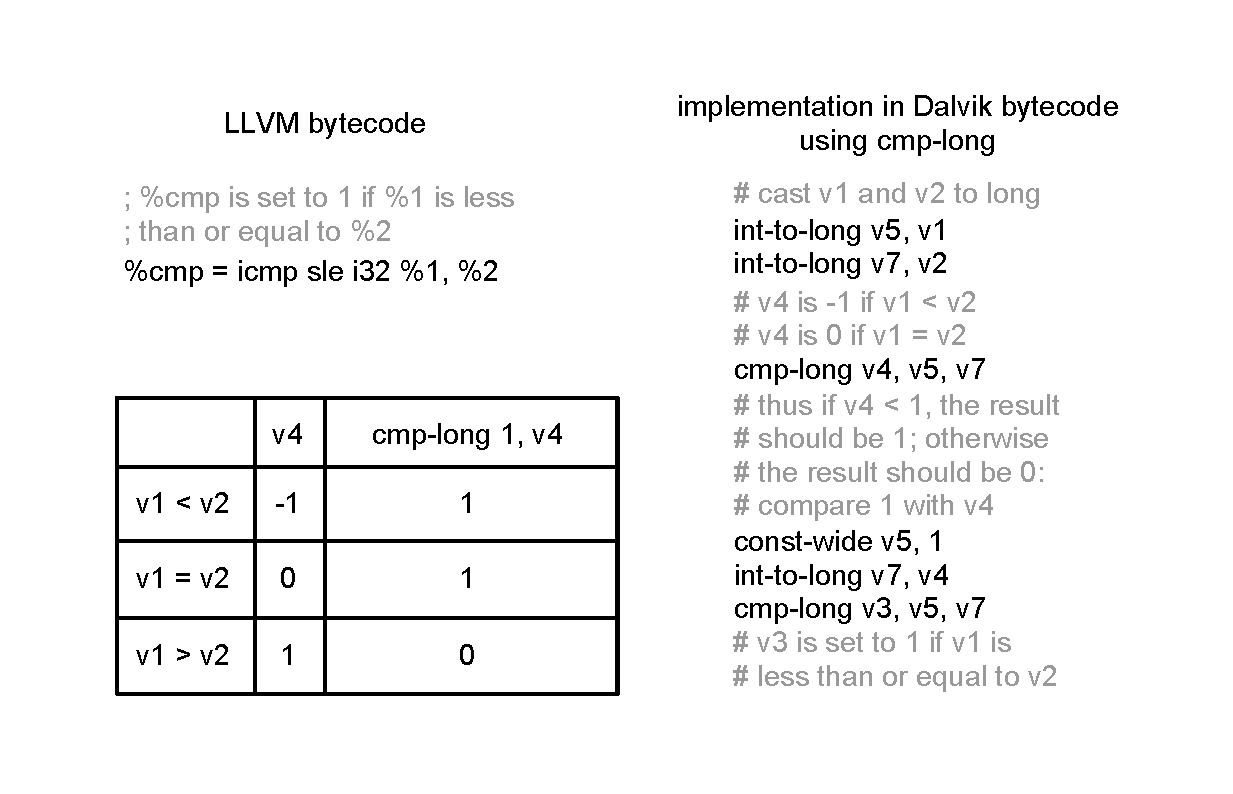
\includegraphics[width=1.0\textwidth]{cmpsle}
    \caption{Translating the LLVM 'icmp sle' instruction variant to Dalvik bytecode.}
    \label{fig:cmpsle}
\end{figure}

To simplify the explanation, call \%1 in the LLVM code and v1 in the Dalvik code A, \%2 in the LLVM code and v2 in the Dalvik code B, and \%cmp in the LLVM code and v3 in the Dalvik code C. The LLVM instruction shown in the figure will return 1 (i.e. C will be 1) if A is less than B, or equal to B, and will return 0 (i.e. C will be 0) if A is greater than B.

On the Dalvik side - when A and B are compared, the result will be -1 if A is less than B, 0 if A is equal to B, and 1 if A is greater than B. Thus, in order to reduce the possible results to two another comparison needs to be performed. The solution is to compare the result of the first comparison with the number one, where one is the first argument. This will produce 1 if the result of the first comparison is -1, or 0, i.e. if A is less than or equal to B, and 0 if the result of the first comparison is 1, i.e. A is greater than B.

At the end, by observing the last column in the table in Figure \ref{fig:cmpsle}, it can be concluded that the results of the LLVM code and the Dalvik code agree. However, it is obvious that his translation is quite verbose, producing six instructions to emulate a single one. This is partly due to the need of casting integers to long integers everytime they need to be compared, which should not be necessarry.

The conversion of the 'less-than' comparison is shown in Figure \ref{fig:cmpslt} as a next example.

\begin{figure}[h!]
    \centering
        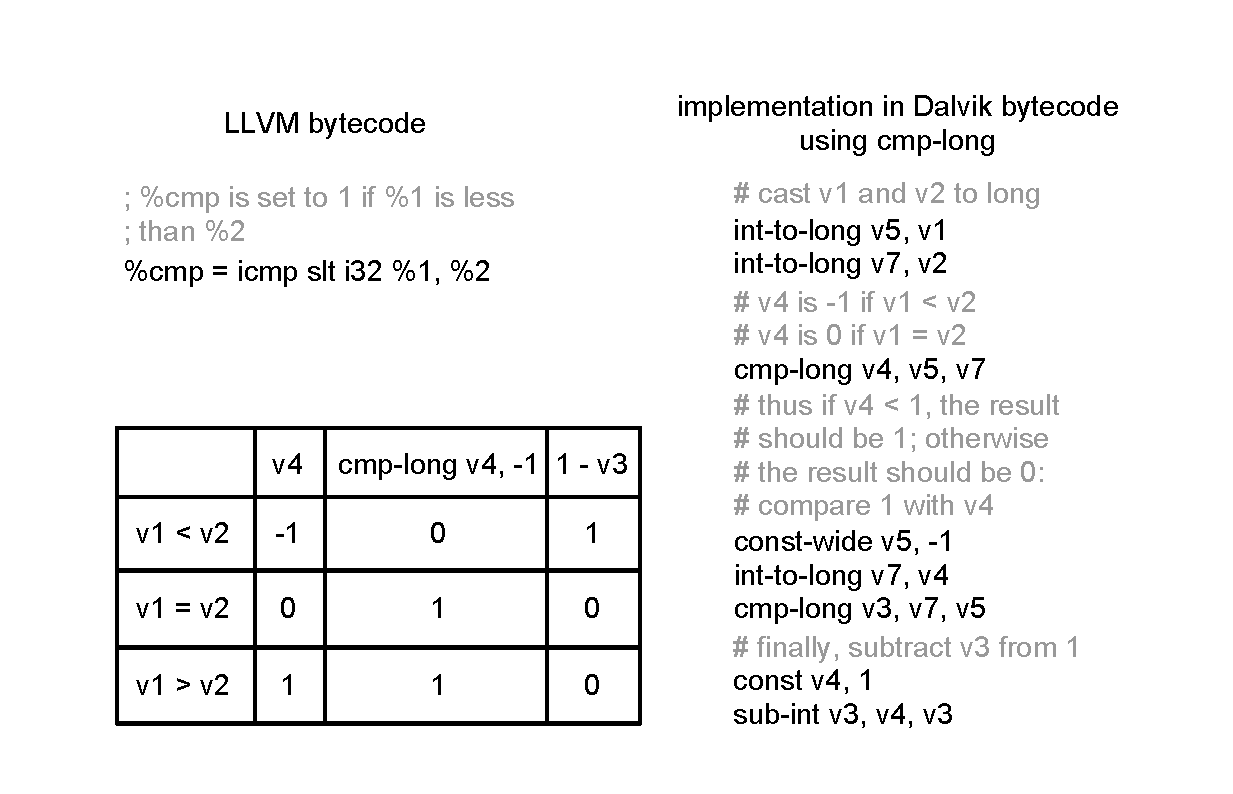
\includegraphics[width=1.0\textwidth]{cmpslt}
    \caption{Translating the LLVM 'icmp slt' instruction variant to Dalvik bytecode.}
    \label{fig:cmpslt}
\end{figure}

During the construction of this translation an important realisation occured to the author: there is no way to have 0 as a result for two of the cases after the second comparison, as this would mean that two different numbers (say, 0 and 1 as in the figure) are equal to the same thing, which is impossible. A way around this complication is to output the code for the negation of the comparison (in this case greater than or equal) and then negate the result. However, this is starting to get suspiciously complicated and at this point the author started to doubt whether this is the better approach.

Considering the example of equality comparison, it becomes clear that using the Dalvik comparison instructions is not the way to go. As can be seen from the table in Figure \ref{fig:cmpeq}, there is no way to implement the LLVM equality comparison in the same fashion as in the previous two examples. A possible option is to use the disjunction of less than or equal and greater than or equal, but this is suboptimal. This lead to the exploration of the other approach.

\begin{figure}[h!]
    \centering
        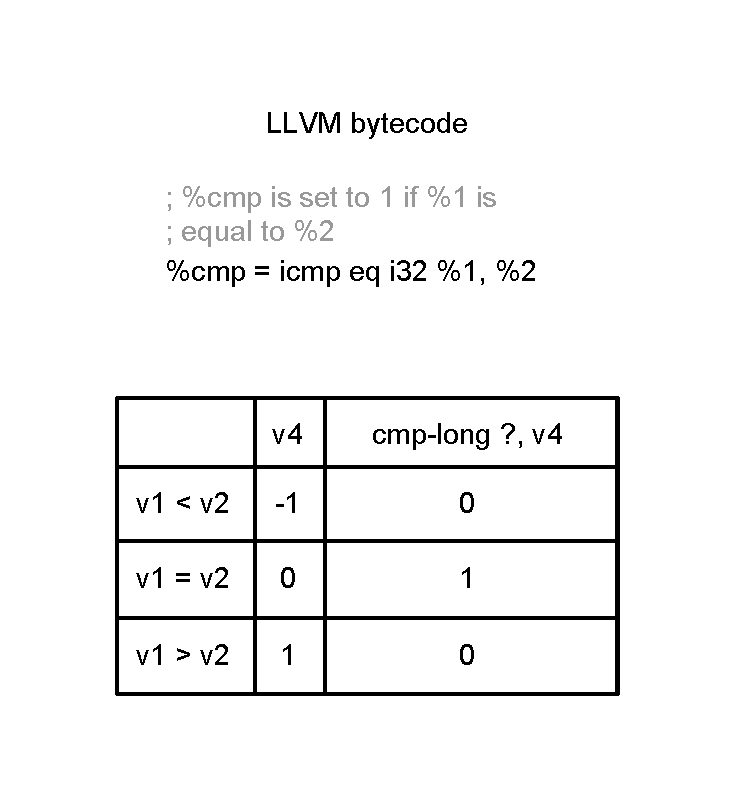
\includegraphics[width=0.6\textwidth]{cmpeq}
    \caption{Translating the LLVM 'icmp eq' instruction variant to Dalvik bytecode. There is no such number that can be used in the comparison, in order to get the necessary result.}
    \label{fig:cmpeq}
\end{figure}

\paragraph{Conditional branches approach} Using conditional branches to implement boolean comparison is not as exciting as using the comparison functions in Dalvik, but it works. Also, as demonstrated by Figure \ref{fig:cmpsle2}, it is not too complicated, and it is definitely easier to understand and shorter than the other approach.

\begin{figure}[h!]
    \centering
        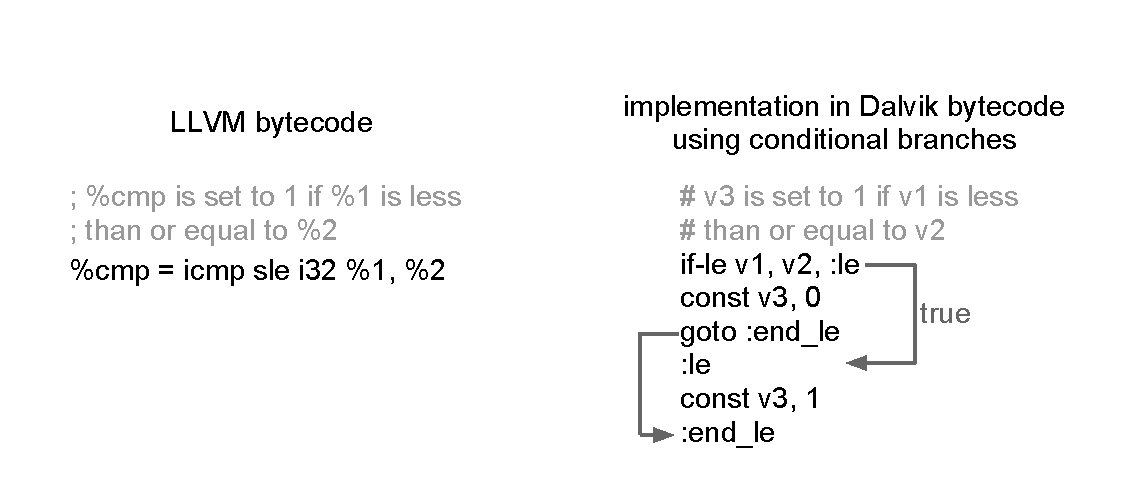
\includegraphics[width=1.0\textwidth]{cmpsle2}
    \caption{Translating the LLVM 'icmp sle' instruction variant to Dalvik bytecode using conditional branches.}
    \label{fig:cmpsle2}
\end{figure}

Thus, the final conclusion of this comparison is that the better and correct way to implement the LLVM comparison instructions, without resorting to writing a library class, is by using the conditional branches in the Dalvik bytecode. Unfortunatelly, due to lack of time, this could not be implemented in the prototype, so the performance implications of this choice are not evaluated. However, disassembling applications compiled by the Android Development Toolkit (ADT), shows that this is the approach taken from the toolkit as well, which is supportive to this conclusion.

\paragraph{The 'br' instruction} "... is used to cause control flow to transfer to a different basic block in the current function. There are two forms of this instruction, corresponding to a conditional branch and an unconditional branch."\cite{P11} The two forms have respectively three and one operands. In the case of a conditinal branch, the first operand is a boolean expression, the second is the label to branch to if the expression is satisfied, and the third is the label to branch to if the expression is not satisfied.

Due to time restrictions, and to keep the prototype simple, the author has implemented conditional branches only for expressions that are a monomial, i.e. a single register or a constant. Thus, this instruction is simulated by printing out the Dalvik 'if-nez' instruction with the translated register and the 'ifTrue' label as arguments. This instruction compares its first argument with zero and if it is different jumps to the specified label.

Then a 'goto' instruction (unconditional branch) is printed with the 'ifFalse' label. The logic is that if the condition is 'false', the program will not branch and the 'goto' instruction will be executed. If the condition is 'true', then the program will branch and the unconditional jump will not be executed.

The unconditional version of 'br' is implemented as a single 'goto' statement.

\paragraph{The 'call' instruction} "... represents a simple function call."\cite{P11} However, this description in the language manual is rather ironic, as 'call' is arguably the most complicated instruction. It can have different markers applied to it, for example indicating whether the callee function is 'tail' (it does not access the stack of the caller), or specifying which caller convention should the caller use. Some of these markers are for optimisation purposes, while there isn't enough control in the Dalvik bytecode to implement others. The author again decided to favour simplicity and implement only the most basic function call. Full support of this instruction can only be achieved by implementing a dedicated library class, or in an interpreter.

The 'call' instruction needs to have the type and the name of the function to be called as arguments. Since functions in the result have the same names as functions in the source, only the type has to be converted to a Dalvik type. This is done according to Table \ref{tab:typeConvertion}. Then, the arguments need to be parsed. Each argument that is a constant is loaded to a temporary register, and each argument that is an LLVM register is translated to a Dalvik register. The next step is to print an invoke-static instruction (as functions are implemented as static methods as explained in section \ref{sec:ModulePassClass}). It specifies the arguments, the name of the callee function, and its type. Finally, the temporary registers (if any) are deallocated and a 'move-result' instruction (an instruction that stores the returned value to a register) is printed.

\chapter{Related Work}

\section{LLJVM}

LLJVM is another project build on top of LLVM. The project was originally made available to the public around November 2009 \cite{P12}, development died out about a year later \cite{P13}, and is not maintained any more.

Its aim is to provide a way of running C code on a Java Virtual Machine. The approach is quite similar to the one taken with Objective-Droid: source code is compiled to LLVM bytecode, then it is ran through the LLJVM backend to produce Jasmin (assembly language for Java), and it is linked and assembled. Just as a remainder for the reader: in Objective-Droid Objective-C code is compiled to LLVM bytecode, then translated by the backend to smali code, linked and assembled.

Unfortunatelly, the author could not build the LLJVM project from source, as it depends on a very specific LLVM version (2.7) which proved quite hard to build on the testing configuration of the time. Other attempts have revealed that the LLJVM code is not compatible with newer versions of LLVM, in particular 3.2. Furthermore, there is no compiled version available, and thus it could not be tested properly. However, from the web page of the project (and the positive comments on it) it appears that the project was at least partially successful.

\section{NestedVM}

Another C-to-Java compiler is NestedVM. In contrast with LLJVM, it relies on gcc, rather than on LLVM, and uses MIPS assembly code as intermediate representation \cite{AllietMegacz:ivme:2004}. It can also target the Java language, which makes it more flexible than LLJVM and Objective-Droid. According to the paper that introduces NestedVM, it is novel in not using native interfaces like JNI to produce Java bytecode from a C program.

NestedVM is an impressive effort, as it provides a runtime that implements a lot of mechanisms found in C programs that are not straightforward to translate to Java, including: unsigned numbers, file I/O, process-level memory management, and syscalls. There is an even more advanced version of the runtime that emulates a large portion of the POSIX API, notably: maintaining filesystems and device nodes, multiprocessing, and simple networking support. Another interesting feature is that the 64KB limit on the size of Java methods is overcome by splitting long programs to multiple methods and linking them together (called trampoline transformation in the paper.)

The paper reports only three to ten times performance reduction when compared to native execution, and claims that this makes NativeVM an attractive solution for code which is not performance-critical.

Objective-Droid is not as complex as NestedVM, as the goal of the project is not to create a complete system, but rather a prototype that shows that it is possible to run Objective-C programs on Dalvik. For this reason many of the features available in NestedVM are not implemented in Objective-Droid[TODO: , but it is still possible to compare their performance, as shown in the evaluation section.]

\chapter{Evaluation}

\section{Correctness}

It is correct.

\section{Performance}

\chapter{Conclusions}

% use the following and \cite{} as above if you use bibtex
% otherwise generate bibtem entries
\bibliographystyle{plain}
\bibliography{final}

\end{document}